%% ==========================================================================
%% SECTION 3: EMPIRICAL EVIDENCE (moved before formal framework)
%% ==========================================================================
\section{Epistemic Observability}\label{sec:empirical}

The formal impossibility we present rests on a premise: that the internal state
of a language model carries epistemic information not exported through the
text-only interface. In systems terms, the model is \emph{unobservable}: it
maintains internal state that affects output correctness but is invisible to
external consumers. Before formalizing this constraint, we demonstrate
empirically that the premise holds because the model's internal geometry distinguishes
what the interface conceals.

We demonstrate the premise in two stages. First, topological analysis of
hidden-state activations in OLMo-3~\cite{olmo2025olmo3} shows that the model's
internal geometry distinguishes grounded from fabricated generation, with
fragmentation scores differing by an order of magnitude across epistemic
conditions (adversarial truths, plausible fabrications, ungrounded lies, and
counterintuitive facts). The same confident, fluent text emerges regardless of
whether the underlying representation is stable or shattered. The formal
impossibility results do not depend on this particular operationalization; the
topological analysis serves only to make the theoretical constraint vivid.

Second, and more importantly, we test whether these internal signals
\emph{detect} epistemic grounding across architectures, not merely correlate
with it in one model.

\subsection{Signal Calibration: From Difference to Detection}

The existence of an internal signal difference does not imply detection. The distinction
matters. We are not claiming the tensor predicts correctness because a model can be
confidently wrong or uncertainly right. We claim the tensor reveals whether the
model is operating in \emph{grounded mode} (retrieving from stable
representations) versus \emph{fabrication mode} (generating without anchoring).

We test this using a taxonomy of query types: \emph{knowable} queries (facts the
model should have stable representations for) versus \emph{unknowable} queries
(fabrication prompts, future events, private information). For each query, we
extract tensor signals during generation: token entropy, top-$k$ probability
mass, and log-probabilities. We then compute ROC curves for each signal's
ability to discriminate knowable from unknowable queries.

Results across four model architectures (Qwen3 4B, OLMo-3 7B, Llama-3.1 8B,
Mistral 7B), pooling 800 query--response pairs:

\begin{itemize}
\item Mean entropy: AUC = 0.870
\item Top-5 probability mass: AUC = 0.881
\item Mean log-probability: AUC = 0.868
\end{itemize}

All three signals are strong classifiers. Effect sizes are large: Cohen's
$d = 1.57$ for entropy (knowable mean = 0.24, unknowable mean = 0.61).

Critically, the direction is consistent across all four architectures:
unknowable queries produce higher entropy in every model tested. This suggests
the signal is architectural rather than an artifact of any particular training
procedure.

A negative result is equally informative. When we test whether entropy predicts
\emph{correctness} (using TruthfulQA's correct vs.\ incorrect answer pairs), AUC
drops to approximately 0.53, which is no better than random. The tensor does not tell
you if the model is \emph{right}. It tells you if the model is operating in a
mode where it \emph{could be} right, because it has something to retrieve rather
than fabricate.

This is the bridge between \autoref{sec:empirical}'s descriptive finding and
\autoref{sec:escape}'s architectural prescription: the escape condition is
not vacuous. Current architectures carry signals that distinguish grounded from
ungrounded generation. They simply discard these signals at the interface.

\subsection{Baseline Comparison: Why the Tensor?}

If simpler methods achieve equivalent discrimination, the tensor interface adds
complexity without benefit. We compare tensor signals against three baselines:

\paragraph{Baseline 1: Self-Reported Confidence.}
Ask the model ``How confident are you in that answer?'' after generation.
This tests whether the model can introspect and report its own epistemic state
through the text channel.

\paragraph{Baseline 2: Hedging Language Detection.}
Count hedging markers (``I think,'' ``possibly,'' ``might be'') and refusal
markers (``I don't know,'' ``cannot verify'') in the response.

\paragraph{Baseline 3: Response Length.}
Use output length as a proxy for uncertainty, on the hypothesis that uncertain
responses may be unusually short (refusal) or long (padding).

Results are stark. Across 800 query--response pairs, tensor signals
substantially outperform text baselines: log-probability AUC = 0.87, entropy
AUC = 0.87, top-5 mass AUC = 0.88. The text baselines fare worse: hedging
language achieves AUC = 0.74, response length AUC = 0.57.

The self-report baseline is particularly instructive. When asked ``How confident
are you?'' after generating, the model reports \emph{higher} confidence on
unknowable queries than on knowable queries. The self-report AUC is below
0.5, which is worse than random, because the relationship is \emph{inverted}. The model
does not merely fail to report its epistemic state honestly; it systematically
misreports, claiming greater confidence precisely when it is fabricating.

Critically, this inversion is \textbf{universal across architectures}. We tested
self-reported confidence across four model families:

\begin{itemize}
\item OLMo-3 7B: Tensor AUC = 0.894, Self-report AUC = 0.284
\item Llama-3.1 8B: Tensor AUC = 0.922, Self-report AUC = 0.330
\item Qwen3 4B: Tensor AUC = 0.896, Self-report AUC = 0.332
\item Mistral-7B: Tensor AUC = 0.905, Self-report AUC = 0.362
\end{itemize}

Every model tested shows the inversion: self-report AUC below 0.5, tensor AUC
above 0.7 (\autoref{fig:entropy_dist}, \autoref{fig:confidence_dist}). The
tensor advantage ranges from +0.53 to +0.61 across architectures.
This universality is notable: the \emph{interface problem} (text misrepresenting
internal state) is architectural, not an artifact of any particular training
procedure or model family.

This confirms the core premise of our impossibility theorems: the model cannot
be trusted to honestly report its own epistemic state through the text channel.
The text is testimony, which is what the model generates. The tensor is
telemetry, which are measurements of the computation that produced the output. The model
can control its testimony; it cannot control its telemetry.

The baseline comparison justifies the complexity of the tensor approach.
Text-based heuristics partially work (hedging language is informative), but
self-report fails catastrophically and universally. Only the tensor provides
reliable access to the epistemic state the model cannot help but reveal through
its computation.

% TODO: Add figure environments once figures are prepared
% TDA figures available in supplementary materials:
% figures/mallku_heatmap.png, mallku_phase_space.png, mallku_topology_scan.png

\begin{figure}[t]
  \centering
  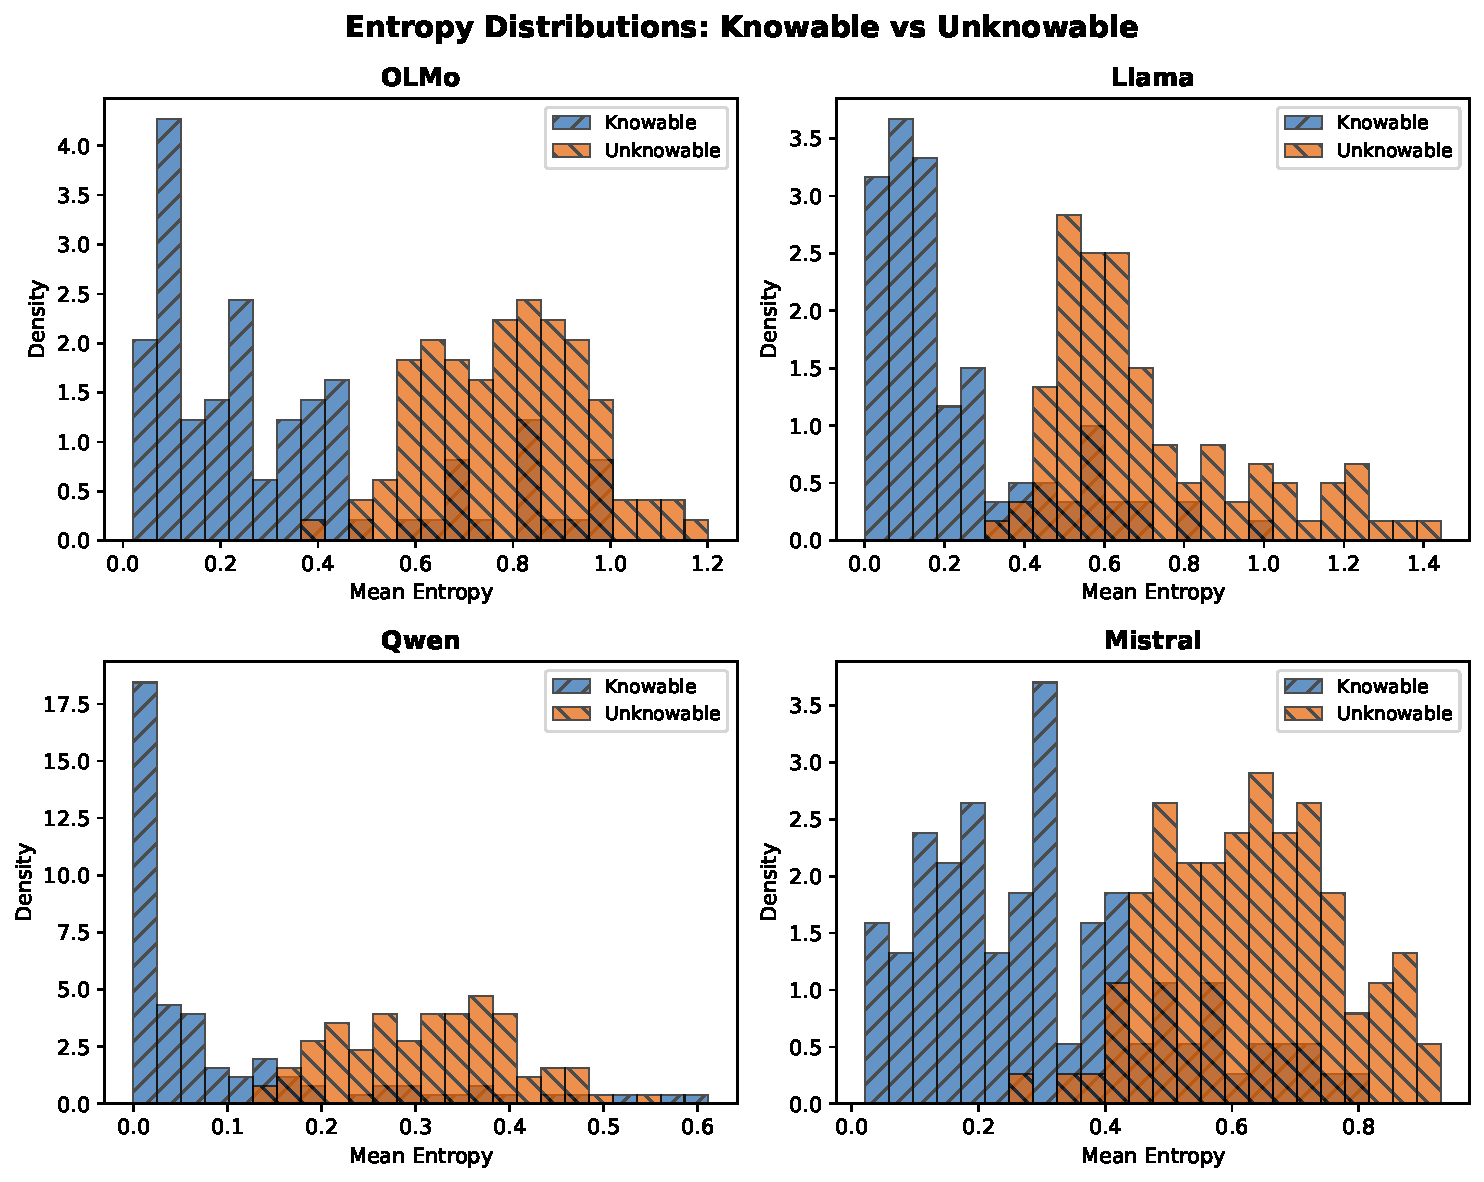
\includegraphics[width=\columnwidth]{figures/exp27_entropy_distributions.pdf}
  \caption{Distribution of mean per-token entropy for knowable vs.\ unknowable
    queries across four model architectures. The distributions are separable in
    every model tested, confirming that entropy discriminates epistemic
    grounding from fabrication at the architectural level.}
  \label{fig:entropy_dist}
\end{figure}

\begin{figure}[t]
  \centering
  
\includegraphics[width=\columnwidth]{figures/exp27_confidence_distributions.pdf}
  \caption{Distribution of self-reported confidence for knowable vs.\ unknowable
    queries. The inversion is universal: every model reports higher confidence on
    unknowable queries than on knowable ones. The distribution is bimodal: 61.3\%
    of unknowable queries receive confidence = 1.0, compared to 19\% of knowable
    queries.}
  \label{fig:confidence_dist}
\end{figure}
